%\subsection{Segmentation de l'environnement intérieur}
%segmentation par l'utilisateur
%\subsection{Création d'une base de connaissance}
%utilisation opencv
%creation du dictionnaire
%calcul du descripteur des objets -> detail sur le nombre d'objet et sur le nombre d'exemplaire
%test sur une base composé de mesh et sur une autre composé de nuage de point
%\subsection{Reconnaissance des objets} 
%simple comparaison avec le descripteur
%TODO voir ce qu'on peut mettre dans cette section

\subsection{Objectif}
%interface
Le but de cette seconde application est de pouvoir modifier un environnement intérieur au travers d'une interface
simple et intuitive. 
Pour cela, nous allons dans un premier temps récupérer un nuage de points d'une pièce intérieure. Puis à partir
de ce nuage de points, nous allons segmenter la pièce afin de pouvoir détecter des objets à l'intérieur de celle-ci.
L'utilisateur doit ensuite sélectionner un objet, ce qui déclenchera l'apparition d'une liste contenant un ensemble de modèle 3D
d'objets équivalents à celui sélectionné. L'utilisateur n'a plus qu'à choisir l'objet qui lui convient dans la liste,
afin de l'ajouter dans un autre environnement 3D présent dans l'application.\\

Lors de ce scénario, nous pouvons voir qu'il y a deux grandes étapes qu'il faudra réaliser dans l'application. Tout d'abord, il faut 
segmenter le nuage de points de la pièce, dans le but de détecter des objets. Puis il faut reconnaître les objets détectés afin
d'afficher la bonne liste d'objets 3D. Nous avons décidé, pour faciliter le développement, de laisser l'utilisateur sélectionner
l'objet qu'il souhaite dans le nuage de points, afin de ne pas avoir à développer la détection d'objet dans le nuage de points.
Pour cela, nous nous inspirons des travaux de T. Shao et al\cite{interactiveSeg} et de J. Xiao et al\cite{interactionSeg2}.
Il nous reste donc à reconnaitre l'objet sélectionné par l'utilisateur.

\subsection{Création de la base d'apprentissage}
Afin de pouvoir reconnaître un objet, nous avons besoin d'un base d'apprentissage contenant les descripteurs d'un ensemble
d'objets. Pour créer cette base, nous utilisons la représentation du \og bag of word \fg ainsi que la méthode d'apprentissage 
automatique SVM\cite{SVM} disponible dans la librairie opencv. Pour la création de notre base, nous utilisons une vingtaine
d'images de six objets différents. Les nuages de points dont nous nous sommes servis pour la création de notre base viennent de 
K. Lai et al\cite{Base1} issue de M. Firman\cite{generalBase} qui a regroupé un ensemble de bases d'objets provenant de caméra 3D.
La base que nous utilisons est composé de plusieurs exemplaires de chaque objet, et chaque exemplaire d'objet est représenté par 
plusieurs images représentant plusieurs angle de vue de l'objet. L'acquisition des objets a été réalisé avec une caméra 
Kinect v1.\\

Le descripteur que nous utilisons pour cette application est le descripteur FPFH\cite{FPFH} qui est l'un des plus efficaces dans la
reconnaissance d'objet à partir de nuage de points. Nous calculons ce descripteur sur l'ensemble des images de notre base afin de
créer le dictionnaire de notre \textit{bag of words}. A cette étape du développement, nous avons créé le dictionnaire, il faut
alors recalculer le descripteur sur chacun des objets afin de déterminer les caractèristiques de chaqu'un d'entre eux. Cela nous
permet d'obtenir un histogramme pour chaque objet comportant les caractèristiques qu'il contient et le nombre de fois où il
apparaît. Il ne reste plus qu'à utiliser le descripteur du \textit{bag of word} dans SVM afin de finaliser la création de 
notre base d'apprentissage. Notre base d'apprentissage est donc un vecteur d'une taille égale au nombre de classe, donc six, 
composé d'histogramme dont la taille est égale au nombre de caractèristique.

\begin{figure}[!ht]
  \begin{center}
    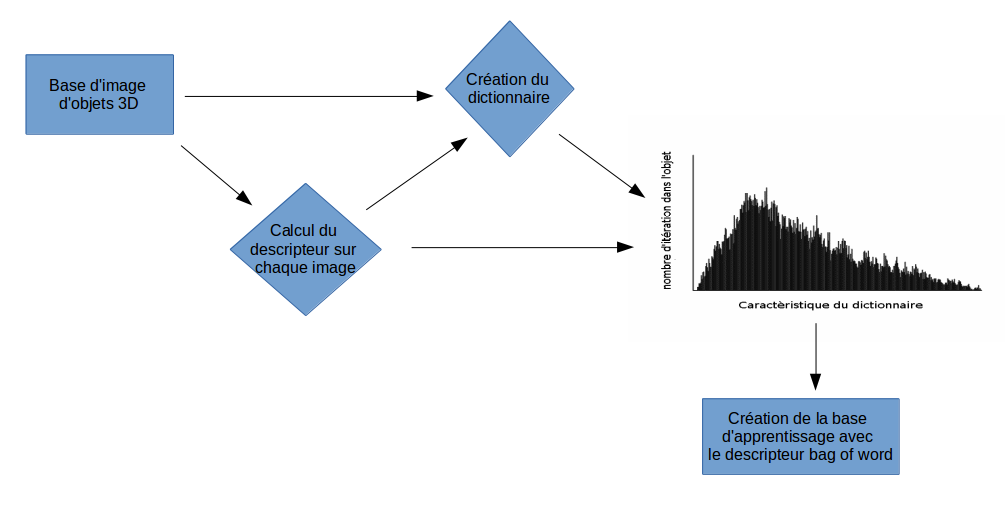
\includegraphics[height=8cm]{image/schemaBase.png}
    \caption{Schéma de la création de la base d'apprentissage}
  \end{center}
\end{figure}

\subsection{Interface utilisateur}
L'interface utilisateur comprend deux fenêtres. La première comporte une vue avec le nuage de points récupéré à partir de la Kinect
et un ensemble d'options. Parmi ces options, nous avons la navigation dans le nuage de points et le choix de la technique de 
sélection. La première sélection est une simple sélection rectangulaire où l'ensemble des données à l'intérieur d'un rectangle formé
par deux points est sélectionné. La seconde est une sorte de pinceau sélectionnant les données en dessous de la souris, ainsi que celles dans 
un voisinage prédéfini autour de celle-ci. Lorsque l'utilisateur a sélectionné un objet et que l'application l'a reconnu, un nombre \textit{n} de cases 
avec des objets apparaît. Les objets dans ces cases sont les mêmes que l'objet sélectionné. Lorsque l'utilisateur clique sur l'une 
de ces cases, l'objets correspondant est ajouté dans la seconde fenêtre.
La seconde fenêtre contient l'environnement final dans lequel il y a déjà une piéce modèlisée avec des objets 3D. L'objet sélectionné est ajouté dans cette environnement. Il est ensuite possible de déplacer l'objet dans l'environement virtuel en
cliquant dessus afin de le positionner à l'endoit voulu dans la pièce.

\begin{figure}[!h]
  \begin{center}
    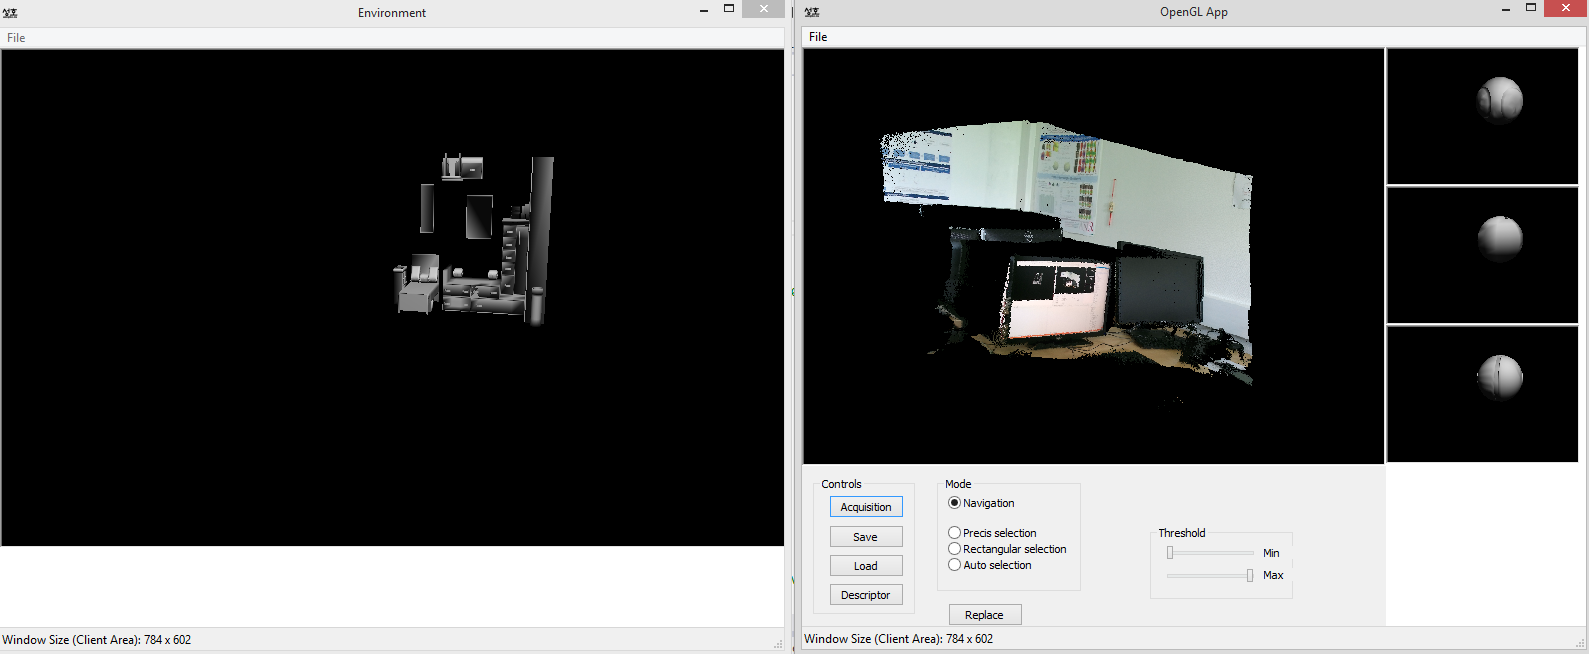
\includegraphics[height=7cm]{image/appliObjet.PNG}
    \caption{Interface de la seconde application}
  \end{center}
\end{figure}

\begin{figure}[!h]
  \begin{center}
    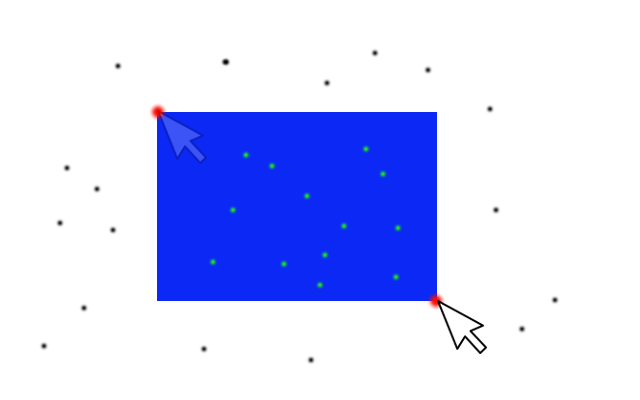
\includegraphics[height=4.5cm]{image/selection1.png}
    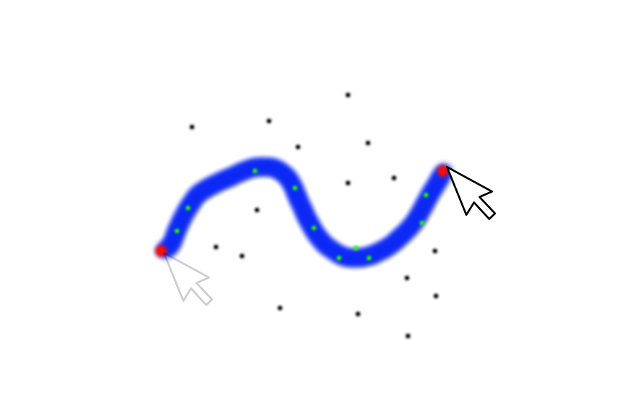
\includegraphics[height=4.5cm]{image/selection2.png}
    \caption{Schéma des deux type de sélection disponible dans l'apllication. Les points verts
    sont les points sélectionnés et en noire les autres.}
  \end{center}
\end{figure}

\subsection{Reconnaissance d'objet}
%TODO parler des résultats de la reconnaissance
Une fois que la base d'apprentissage et l'interface créé, nous ajoutons le code de la reconnaissance de forme dans l'application.
Pour cela, nous filtrons les données que l'utilisateur à séléctionné. Nos méthodes de sélection n'étant pas très précise, il arrive
courrament que l'utilisateur sélectionne du bruit ou des parties de l'environnement. Pour filtrer les données nous utilisons
les deux mêmes classe que dans l'application précédente, c'est-à-dire \textit{StatisticalOutlierRemoval} et \textit{VoxelGrid}.
Lorsque le filtrage est réalisé, il nous faut calculer le même descripteur que dans notre base sur les données sélectionné par 
l'utilisateur et envoyer le résultat dans notre SVM afin qu'il détermine la classe de l'objet.

\subsection{Travaux futures et applications}
L'application final de ce projet est assez complète et très fonctionnel, cependant il existe plusieurs extansion qu'il 
est possible d'ajouter au projet. Par exemple notre liste d'objet proposé à l'utilisateur pour l'ajouter à la 
scène 3D n'est pas assez conséquente. Nous pourrions ajouter plus d'objet en récupérant une base venant de grand magasin
de meuble par exemple. Ainsi l'utilisateur pourrait potentiellement retrouver le meuble qu'il a scanné. Cela pourrait
déboucher sur une application beaucoup plus importante, où l'environnement dans lequel nous souhaitons ajouter des meubles
représente la future maison d'une personne. Si cette personne souhaite voir comment elle pourrait placer ces meubles dans 
son prochain investissement, elle n'aurait cas récupérer un modèle 3D des lieux et scanner l'ensemble de ces meubles pour
les ajouter dans la scène.
